\documentclass[
	english,
	fontsize=10pt,
	parskip=half,
	titlepage=true,
	DIV=12
]{scrartcl}

\usepackage[utf8]{inputenc}
\usepackage{babel}
\usepackage[T1]	{fontenc}
\usepackage{lmodern}
\usepackage{microtype}
\usepackage{color}
\usepackage{csquotes}
\usepackage{tabto}

\usepackage{hyperref}

\usepackage{graphicx}
\usepackage{wrapfig}
\usepackage[bf]{caption}
	\captionsetup{format=plain}

\newcommand*{\tabcrlf}{\\ \hline}

\usepackage{amsmath}

\usepackage{minted}
	\usemintedstyle{friendly}

\newcommand*{\inPy}[1]{\mintinline{python3}{#1}}
\newcommand*{\ie}{i.\;e. }
\newcommand*{\eg}{e.\;g. }

\newcommand{\thus}{\ensuremath{\rightarrow}}

\begin{document}

\part*{Python Problems 05, Winter 2021/22}
\section{Cross Sum (1\;P)}
Write code that takes an integer as input and computes the cross sum of this number.


\section{Fizzbuzz (1 + 1\;P)}
In the Game \emph{FizzBuzz}, players count from one upwards. If a number is divisible by three, the player should not name the number, but say \emph{fizz}. If the number is divisible by five, players should say \emph{buzz}. If the number is both, divisible by three and five, players say \emph{fizzbuzz}. Hence, players count like this:
\begin{center}
	1, 2, fizz, 4, buzz, fizz, 7, 8, fizz, buzz, 11, fizz, 13, 14, fizzbuzz ...
\end{center}

Create a program that puts this sequence on the screen.

\emph{Optionally: (+1 P)}\\
Write your code such that the rules can be expanded easily. Make it such that you can easily change the divisors and the replacement words. It is possible to write your code such that adding a single line adds, for example, the rule: \emph{numbers divisible by seven are replaced by \enquote{tezz}}.


\section{Text To List (1\;P)}
Write a program that takes a string of numbers separated by commas and that computes a \inPy{list} containing the numbers from this.

\emph{Example}:\\
Input: \inPy{"1, 5, 99, -3, 5.7"} \tab
Output: \inPy{[1, 5, 99, -3, 5.7]}

\emph{Hint:} This can be done with a single line of code.


\section{Line Breaks (3\;P)}
Create a text variable that stores one line of long text. Create another \inPy{int} variable \texttt{width} that specifies how many characters fit in one line. With these two inputs, write an algorithm that prints out your text variable as several lines. None of these printed lines should be longer than \texttt{width} characters, and no words should be split.

Example:\\
The input
\begin{minted}{python3}
text = 'We shall say "Ni" again to you, if you do not appease us.'
width = 20
\end{minted}

should produce the output:
\begin{minted}{text}
We shall say "Ni" 
again to you, if you 
do not appease us.
\end{minted}


\section{Integral (I) (1 P)}
\begin{wrapfigure}{r}{.3\linewidth}
	\vspace{-50pt}
	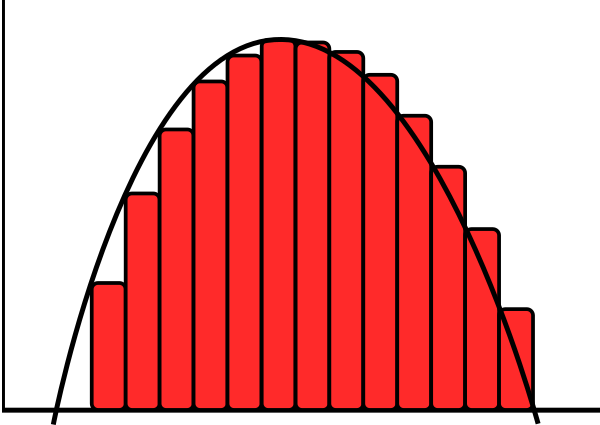
\includegraphics[width=\linewidth]{./integral}
	\caption{Approximation of an integral by area of rectangles.\newline
		Figure by Jonas Süskind}
	\vspace{-30pt}
\end{wrapfigure}
Write a function \texttt{integrate} that approximates the area underneath a graph of a function $f$, \ie compute the value
\[ \int_a^b f(x) \;\text{d}x \]

The integrand $f$ (\ie the function that gives the graph) should be a parameter to your function \texttt{integrate}. Make it such that your function has the signature:
\mint{python}{def integrate(func, start, stop, N) :}

Use the rectangle approximation:
\begin{itemize}
\item Disect the integration interval into $N$ blocks of equal width
\item For each block, evaluate the function $f$ at the left hand side of your block. This gives the height of the rectangles
\item Find the areas of all $N$ rectangles and sum them up -- this gives you an approximation of the integral
\end{itemize}

You can test your code with the following call:
\mint{python}{print( integrate(math.exp, 0, 1, 10000) )}
The output should, approximately, be \texttt{1.718}.

\end{document}
